\documentclass[12pt]{article}
\usepackage[]{graphicx}
\usepackage[]{color}
\usepackage{amsmath, amsfonts, amssymb, amsthm, latexsym}
\usepackage{multicol}
\usepackage{graphicx}
\usepackage{longtable}
\usepackage{titlesec}

%\usepackage{tikz, MnSymbol}
%\usetikzlibrary{arrows,shapes,positioning}
%\usepackage{float}
%\usepackage{pstricks}
%\usepackage{setspace}

\usepackage[margin=2.4cm]{geometry}
\setlength{\parindent}{0cm}

\setcounter{secnumdepth}{4}

\titleformat{\paragraph}
{\normalfont\normalsize\bfseries}{\theparagraph}{1em}{}
\titlespacing*{\paragraph}
{0pt}{3.25ex plus 1ex minus .2ex}{1.5ex plus .2ex}

\providecommand{\ds}{\displaystyle}
\providecommand{\abs}[1]{\left\vert#1\right\vert}
\newcommand{\given}{\hspace{3pt}|\hspace{3pt}}
\newcommand{\blip}{\hspace{2pt}}

\begin{document}
{\Large {\bf Summary}}\\
This report describes population model analyses done in support of the evaluation of management actions for pallid sturgeon on the Upper Missouri River, from Fort Peck Dam to Lake Sakakawea, using a deterministic population projection matrix.  The particular management actions of focus were alternative flow release protocols from Fort Peck Dam.  Seven alternative scenarios were considered:  No action, Alternative 1, Alternative 1a, Alternative 1b, Alternative 2, Alternative 2a, and Alternative 2b.  Additionally, potential effects of temperature are explored.   Alternative scenarios were compared in terms of their ability to be fully implemented throughout the period of record (1930-2012), estimated effects on drifting free-embryo retention, and associated long-term growth rates.  Sensitivity and elasticity analyses were conducted to evaluate the effects of parameter values, including uncertainties in age-0 survival and probability of spawning in the Missouri River, on long-term population growth rate. Limitations and uncertainties in the modeling, including the availability of information to parameterize the population model, are discussed.  Important future directions for the population model, such as incorporating fish passage at Intake in the Yellowstone, are also introduced.  

\begin{section}{Introduction}
\end{section}

\begin{section}{Methods}
\begin{subsection}{Modeling Framework \& Spatial Extent}
Seven alternative management scenarios at Fort Peck Dam were considered.   Details of the management scenarios:  No action, Alternative 1, Alternative 1a, Alternative 1b, Alternative 2, Alternative 2a, and Alternative 2b, are described in \textit{REFERENCE HERE}.  Alternative management scenarios were only analyzed during years in which they met alternative-specific flow criteria.  Flow criteria was two-fold: (1) environmental conditions needed to be such that the given alternative hydrograph could be produced (e.g., enough water available for release), and (2) discharge needed to reach a magnitude greater than 20kcfs in order to produce a sufficient spawning cue. For each alternative management scenario and year combination that met flow criteria, long-term population growth rate ($\lambda$) was estimated for the population of pallid sturgeon residing within the Upper Missouri River from Fort Peck Dam to Garrison Dam, including the Yellowstone River up to the Intake Diversion Dam (Figure 1).  The modeling framework used to calculate long-term population growth relied upon several submodels, including hydrological modeling in HEC-ResSim, a spawning model, HEC-RAS drift-dispersion modelling coupled with a free-embryo development model, and a pallid sturgeon demographic population model (Figure 2).  

\begin{subsubsection}{Hydrology, Drift, Development, \& Probability of Retention}
Hydrological data were generated using the Hydrologic Engineering Centers Reservoir Simulation (HEC-ResSim) software implemented for the Missouri River reach between Fort Peck Dam and Lake Sakakawea (see \textit{REFERENCE} for further HEC-ResSim modeling details).  All hydrological runs used for this analysis used historical runoff from the period of record of 1930--2012.  Reservoir operations were modeled for each alternative scenario assuming the same operation rules were in effect for all years.    For each alternative management scenario and year combination that met flow criteria, the probability that a free-embryo develops to settlement prior to reaching the unfavorable conditions of Lake Sakakawea (retention probability) was estimated. The probability of free-embryo retention within the free-flowing Missouri River was computed by integrating a temperature dependent free-embryo development model into HEC-RAS drift simulations, assuming spawning occurs just below Fort Peck dam.  The details of the modeling are described in \textit{REFERENCE HERE}.  Outputs from this modelling provided summary information about development and retention over time, from which the retention probability could be estimated as detailed below.\\

The ``Outputs'' spreadsheet from each of seven HEC-RAS summary workbooks\footnote{e.g., Alt1\_Summary.xlsx}, one for each alternative, were loaded into R.  These spreadsheets contained summary information for each year the given alternative scenario produced the desired hydrograph with a spawning cue discharge greater than 20kcfs, i.e. met flow criteria.  The summary information included the amount of cumulative thermal units (CTUs) expected to be absorbed by the free-embryos and the percentage of free-embryos retained in the free-flowing Missouri River at 3 hours intervals.  A threshold value of 200 CTUs was assumed to indicate transition from drift to settlement (Braaten et al. 2012).  An R script identified the time interval during which the threshold CTU value was surpassed and estimated the retention probability from the given data.  The probability of retention for the year and alternative scenario under consideration, was computed by interpolation, using the CTU and retention data from the endpoints of the identified interval:
\begin{equation}
p_{ret}=\frac{(CTU(t_2)-200)R(t_1)+(200-CTU(t_1))R(t_2)}{CTU(t_2)-CTU(t_1)},
\end{equation}  
where\\
\hspace*{0.5cm}$p_{ret}$ is the retention probability for the year and alternative scenario under consideration,\\
\hspace*{0.5cm}$CTU(t)$ is the estimated cumulative thermal units absorbed by a drifting free-embryo at\\
\hspace*{1.5cm}time $t$,\\
\hspace*{0.5cm}$R(t)$ is the estimated percentage of free-embryos that have been retained in the free-flowing\\
\hspace*{1.5cm}Missouri River at time $t$,\\
\hspace*{0.5cm}$t_1$ is the discrete HEC-RAS time in hours of drift that is associated with the largest CTU\\ 
\hspace*{1.5cm}value that is less than or equal to 200 CTUs, and\\
\hspace*{0.5cm}$t_2$ is the discrete HEC-RAS time in hours of drift that is associated with the smallest CTU\\
\hspace*{1.5cm}value that is greater than 200 (3 hours after $t_1$).\\
\end{subsubsection}

\begin{subsubsection}{Hydrology and Spawning Probability}
The probability a reproductively-ready female spawns within the Missouri River as opposed to spawning within the Yellowstone River or not spawning (atresia)---henceforth referred to as ``Missouri River spawning probability'' or occasionally, simply as ``spawning probability''---was determined by a spawning model.  While there are hypotheses on what factors effect spawning probability, the functional relationship is largely uncertain.  Limited data has shown \textit{FILL IN THIS SECTION}.\\
 
As a first approach, the probability a reproductively-ready female spawns in the Missouri River ($\gamma$) was modeled in terms of discharge and temperature as a multi-variate step function:
\begin{equation}
\gamma(Q, T) = \begin{cases}
\gamma_{high}, & \hspace{0.5cm}  Q\geq Q^{*} \hspace{12pt} \& \hspace{12pt} T\geq T^{*}\\
%\gamma_{med}, & \hspace{0.5cm}  Q\geq Q^{*} \& T_{sp, low} \leq T< T^{*}\\
\gamma_{low}, & \hspace{0.5cm}  Q< Q^{*} \hspace{12pt} \mbox{or} \hspace{12pt} T< T^{*}
\end{cases},
\end{equation}
where\\

\hspace*{0.5cm}$Q$ is the \textit{maximum} discharge \textit{during April--May} in kcfs,\\
\hspace*{0.5cm}$Q^{*}$ is the threshold discharge needed to attract and retain spawners up the Missouri River\\ 
\hspace*{1.5cm}to the vicinity of Fort Peck Dam (in kcfs),\\
\hspace*{0.5cm}$T$ is the maximum temperature reached below Fort Peck Dam during \textit{the end of May--\\
\hspace*{1.5cm}beginning of July} in $^{\circ}$C,\\
\hspace*{0.5cm}$T^{*}$ is the threshold temperature required for spawning (in $^{\circ}$C),\\
\hspace*{0.5cm}$\gamma_{high}$ is the probability that a reproductively-ready female will spawn in the Missouri River\\ 
\hspace*{1.5cm}below Fort Peck Dam given favorable flow and temperature conditions, and\\
\hspace*{0.5cm}$\gamma_{low}$ is the probability that a reproductively-ready female will spawn in the Missouri River\\
\hspace*{1.5cm}below Fort Peck Dam given unfavorable conditions.\\

Baseline values for $Q^{*}$, $T^{*}$, $\gamma_{high}$, and $\gamma_{low}$ were based on observed cases of female spawning migrations up the Missouri River above the confluence with the Yellowstone (Fuller \& Haddix 2013), as well as other spawning data related to temperature (DeLonay et al. 2016) (Table 1).  Outputs from HEC-ResSim provide values for $Q$.\footnote{Craig is this accurate?}  Since alternative management scenarios were only analyzed in HEC-RAS for years in which they could be implemented and the spawning cue discharge exceeded $Q*=20kcfs$, $\gamma=\gamma_{high}$ for the management scenario and year combinations that met flow criteria given $T>T*$.  As a first approach, temperature was assumed to exceed its threshold criteria of $T*=16^{\circ}C$ during each year a management scenario met flow criteria.\footnote{Craig, I wasn't sure how best to assess this criteria given the temperature data available.  I have lots of questions on this I'm hoping we can discuss.  I'll put a few at the end in hopes of sparking some ideas, while I'm away.}   
\end{subsubsection} 

\begin{subsubsection}{Demographic Population Model}
The demographic pallid sturgeon population model is a prebreeding Leslie matrix model:
\begin{eqnarray}
N_{t+1} & = & AN_{t},\\
A & = &  \begin{pmatrix}
F_1 & F_2 & F_3 & \cdots & F_{a_{max}-1} & F_{a_{max}}\\
\phi_1 & 0 & 0 & \cdots  & 0 & 0\\
0 & \phi_2 & 0 & \cdots  & 0 & 0\\
0 & 0 & \phi_3 & \ddots & 0 & 0\\
\vdots & \vdots & \ddots  & \ddots & \vdots & \vdots\\
0 & 0 & 0 & \cdots & \phi_{a_{max}-1} & 0\\
\end{pmatrix},
\end{eqnarray}
where\\
\hspace*{0.5cm}$N_t$ is a vector of population sizes by age-class in year $t$,\\
\hspace*{0.5cm}$A$ is a Leslie matrix,\\
\hspace*{0.5cm}$F_i$ is the expected fertility value of an age-$i$ female pallid sturgeon,\\
\hspace*{0.5cm}$\phi_i$ is the probability that a female survives from age-$i$ to age-$i+1$, and\\
\hspace*{0.5cm}$a_{max}$ is the maximum age of a female fish.\\

The age-specific fertility values are functions of the probability of free-embryo retention ($p_{ret}$) and the probability a reproductively-ready female spawns in the Missouri River ($\gamma$) and vary by management alternatives (Figure 2).  Details of the model parameterization are described in the following three sections with baseline parameter values listed in Table 1.\\

\paragraph{Maximum Age}
The baseline maximum age of a female pallid sturgeon was taken to be 60 years old.  Bratten et al. (2015) estimated the ages of 11 deceased natural-origin pallid sturgeon from the Upper Missouri River.  They determined longevity to be at least 50 years, with individual estimates ranging from 37-59 years old.\\

\paragraph{Age-Specific Survivals}
Age-specific survivals were estimated for pallid sturgeon ages 1 through 9 years old utilizing data from Rotella et al. (2017).  Only data for fingerlings released in RPMA 2 in the Missouri River with an ``IV status'' and ``fin curl status'' of zero were analyzed.  Fingerlings, released into the river at about 3 months old, were chosen with the expectation that having 9 months to acclimate to river conditions would allow for a better estimate of natural age-1 to age-2 survival than yearlings released into the river much closer to their first birthday.\\  

Data tables in Rotella et al. (2017) were provided for each cohort of fingerlings released into the Missouri River and contained information on the estimated number of fish at the start and end of several consecutive interval after release.  Interval periods were not necessarily equal in length, but start and end dates were provided in the tables.  Therefore, for each healthy cohort of fingerlings released, we calculated daily survivals from the data provided in the tables as
\begin{equation}
\mbox{Interval Daily Survial}=\left(\frac{N \mbox{ at Interval End}}{N \mbox{ at Interval Start}}\right)^{1/\mbox{{\scriptsize Days in Interval}}}.
\end{equation}

We then used cohort-specific interval daily survivals to compute cohort-specific survivals from age-class to age-class, assuming all fish were born on June 1st.  The weighted average of cohort-specific annual survivals was used as an estimated for the age-specific annual survivals:
\begin{equation}
\phi_i=\frac{\displaystyle\sum_{c \hspace{1pt} \in \hspace{1pt} C} \phi_{i,c}N_{i,c}}{\displaystyle\sum_{c \hspace{1pt} \in \hspace{1pt} C} N_{i,c}},
\end{equation} 
where\\
\hspace*{0.5cm}$\phi_i$ is the age-$i$ survival probability for ages $i=1, 2, \ldots, 9$,\\
\hspace*{0.5cm}$\phi_{i,c}$ is the probability that a fish in cohort $c$ survives from age-$i$ to age-$i+1$,\\ 
\hspace*{0.5cm}$N_{i,c}$ is the expected number of age-$i$ fish in cohort $c$ on June 1st, and\\
\hspace*{0.5cm}$C$ is the set of all healthy cohorts (IV=0, Fin Curl=0) released into the Missouri River\\ 
\hspace*{1.5cm}within RPMA 2 as fingerlings.\\

Adult annual survival ($\phi_{adult}$) was computed from RPMA 2 wild adult population estimates in 2004 and 2008 (Klungle \& Baxter 2004, Jaeger et al. 2008) as
\begin{equation}
\phi_{adult}=\left(\frac{125}{158}\right)^{1/4}\approx 0.94,
\end{equation}
and set as the survival probability of all females age-15 and older.  Survival probabilities for age-10 to age-14 pallid sturgeon were extrapolated ad hoc from the probabilities computed for younger and older fish (Figure 3, Table 1).\\

  



\paragraph{Age-Specific Fertilities}
Age-specific fertility values ($F_i$) were broken down into several components:
\begin{equation}
F_i=\psi_i\gamma E_ir\phi_{0}p_{ret},
\end{equation}
where\\
\hspace*{0.5cm}$\psi_i$ is the proportion of age-$i$ females that are reproductively ready to spawn,\\
\hspace*{0.5cm}$\gamma$ is the fraction of reproductively-ready females that spawn in the Missouri River, often\\
\hspace*{1.5cm}referred to as ``Missouri River spawning probability'' or ``spawning probability'',\\
\hspace*{0.5cm}$E_i$ is the number of eggs per spawning age-$i$ female,\\ 
\hspace*{0.5cm}$r$ is the sex ratio (fraction of the eggs that are female),\\
\hspace*{0.5cm}$\phi_{0}$ is the survival from egg to age-1 given retention within the free-flowing Missouri\\
\hspace*{1.5cm}River, often referred to simply as ``age-0 survival'', and\\
\hspace*{0.5cm}$p_{ret}$ is the probability a drifting free-embryo is retained in the free-flowing Missouri River.\\

Only age-0 survival is considered for those fish retained in the free-flowing Missouri River ($\phi_{0}$) because it is assumed that survival in the anoxic conditions of Lake Sakakawea is zero.   For the baseline analysis estimating current conditions, it is assumed that retention probability is 1 in 1,000 and spawning in the Missouri River occurs about once every 100 years (Table 1).   In general, both the retention probability ($p_{ret}$) and the probability a reproductively-ready female spawns within the Missouri River ($\gamma$) are assumed to be directly effected by temperature and flow.  Therefore, they vary with environmental conditions, as well as choice of management action.   For the Fort Peck Flows analyses, $p_{ret}$ and $\gamma$ are estimated as outputs of the drift-development and spawning models, respectively, given the particular management alternative scenario and hydrology.  The remaining parameter values ($r$, $\phi_0$, $\psi_i$, and $E_i$) are fixed among scenarios, and described in detail below.\\ 

\textbf{\underline{Sex Ratio and Age-0 Survival}}\\

\vspace{-6pt}Both the probability a fish is female ($r$) and the probability of surviving from egg to age-1 given retention in the Missouri River ($\phi_0$) are constants, independent of the mother's age.  The baseline sex ratio $r$ was computed from a 2008 Upper River (RPMA 2) estimate of 125 wild adults and 40 wild female adults (Jaeger et al. 2008), as
\begin{equation}
r=\frac{40}{125}= 0.32.
\end{equation} 
Missouri River age-0 survival is highly uncertain.  We set baseline Missouri River age-0 survival at an arbitrary, small probability of 75 in 1,000,000 or
\begin{equation}
\phi_0=0.000075.
\end{equation}
We further examine the sensitivity of model outcomes to changes in $\phi_0$.   Additionally, Missouri River age-0 survival likely varies with turbidity, and is an area of future consideration for linking management actions to population outcomes.\\

The probability a female is reproductively ready to spawn ($\psi_i$) and the expected number of eggs released per spawning female ($E_i$) are age-specific quantities.  Their baseline values were determined using multiple steps, as described first for $\psi_i$ and then for $E_i$ below.\\ 

\textbf{\underline{Probability a Female is Reproductively Ready ($\psi_i$)}}\\

\vspace{-6pt}The proportion of age-$i$ females that are reproductively ready is a function of maturation and spawning period:
\begin{equation}
\psi_i = \begin{cases}
m_i, & \hspace{1cm} i=0, 1, \ldots, a_m,\\
m_i + \sum_{j=a_{m}}^{i-1}\psi_{j}p_{i-j},  & \hspace{1cm} i=a_m+1, \ldots, a_{max}\\
\end{cases},
\label{psii}
\end{equation}
with
\begin{equation}
\sum_{i=1}^{a_{max}} m_i=1 \hspace{24pt} \mbox{ and } \hspace{24pt} \sum_{t=1}^{\infty} p_t =1,
\end{equation}
where\\ 
\hspace*{0.5cm}$\psi_i$ is the proportion of age-$i$ females that are reproductively ready to spawn,\\
\hspace*{0.5cm}$m_i$ is the proportion of age-$i$ females that just matured, i.e., the probability that the first\\ 
\hspace*{1.5cm}time a female is reproductively ready to spawn is when she is age-$i$,\\
\hspace*{0.5cm}$p_t$  is the probability that the period of time between being reproductively ready is $t$ years,\\
\hspace*{0.5cm}$a_m$ is the minimum age at which a female matures, and\\
\hspace*{0.5cm}$a_{max}$ is the maximum age of a female fish.\\


The maturation age of female pallid sturgeon has not been well studied and is an area of further informational need (DeLonay et al. 2016).  Age of maturation could also vary by region of the river (George et al. 2012) with observations from the Upper Missouri River suggesting that female pallid sturgeon mature later than those in the Lower Missouri and Mississippi Rivers (Molly Webb, USFWS, personal communication).  The available published data involves only a handful of fish primarily from the Lower Missouri and Mississippi Rivers.   These females were estimated to have matured between the ages of 8 and 20 years old (Keenlyne \& Jenkins 1993, George et al. 2012).  Aging of the fish was typically performed by pectoral fin ray analysis, a method that can suffer from low accuracy and precision (Hurley et  al. 2004). 


We used a logistic cumulative distribution model to describe maturation of females with age:
\begin{equation}
M(a)=\frac{1}{1+e^{-k(a-a_h)}}
\label{cdf}
\end{equation}  
where\\
\hspace*{0.5cm}$M(a)$ is the proportion of age-$a$ females that have reached maturity,\\
\hspace*{0.5cm}$a_h$ is the age at which half of all females are mature,\\ 
\hspace*{0.5cm}$k$ is a scaling parameter that controls the variance of the distribution, and\\
\hspace*{0.5cm}$a$ is age.\\

To account for later maturation ages in Upper River females, we assumed that 50\% of female pallid sturgeon reach maturity by age 15 ($a_h=15$), 5 years later than the expected value used by Wildhaber et al. (2017) for female's in the Lower Missouri River.  We also assumed $k=1$ (corresponding to approximately 5 years representing 3 standard deviations).  We converted this unbounded, continuous cumulative maturation distribution to a discrete probability distribution bounded between the ages of 8 and 21 (Figure 4), as follows: 
\begin{equation}
m_i = \begin{cases}
0, & \hspace{1cm} i=1, 2, \dots, a_m-1\\
M(i), & \hspace{1cm} i=a_m\\
M(i)-M(i-1), & \hspace{1cm} i=a_m+1, a_m+2, \ldots, a_M-1\\
1-M(i-1), & \hspace{1cm} a=a_M\\
0, & \hspace{1cm} i=a_M+1, a_M+2, \ldots, a_{max}
\end{cases},
\label{mi}
\end{equation} 
where\\
\hspace*{0.5cm}$a_m$ is the minimum age at which a female matures,\\
\hspace*{0.5cm}$a_M$ is the maximum age at which a female matures, and\\ 
\hspace*{0.5cm}$M$ is the cumulative distribution described in (\ref{cdf}).\\ 


The spawning period (i.e., the number of years that pass between two consecutive spawning events) of female pallid sturgeon is likely 2-5 years (Delonay et al. 2016), although it has been estimated to be as great as 10 years in past studies using spawning bands (Dryer \& Sandvol 1993, Keenlyne \& Jenkins 1993).\footnote{Assuming no atresia, spawning period and the reproductive-readiness period are equivalent.  Moreover, studies of spawning period often include assessments of reproductive-readiness but do not necessarily confirm spawning.  Therefore, estimates of spawning period also reflect estimates of the number of years that pass between a female being reproductively-ready to spawn.  While admitting it not to be entirely accurate, we occasionally use the terms ``spawning period'' and ``reproductive-readiness period'' (or ``reproductive period'' for short) interchangeably.}  Fuller et al. (2007) and DeLonay et al. (2016) assessed the reproductive-readiness of  28 female pallid sturgeon.  Their data shows that all 28 females had a reproductive period greater than 1 year ($p_1=0$).  Additionally, 8 females had a confirmed spawning period of 2 years with 13 others confirmed as having a spawning period greater than 2 years ($p_2=8/21$).  Of the 13 females whose spawning period was greater than 2 years, only the fates of 5 were known beyond this point: 3 females had a confirmed spawning period of 3 years and 2 females had a confirmed spawning period that was greater than 3 years ($p_3=(13/21)(3/5)$).  Under the following additional assumptions:
\begin{enumerate}
\item the maximum reproductively ready period of a female is 5 years, and
\item a female is approximately twice as likely to have a reproductively ready period of 4 years as she is 5 years,
\end{enumerate}
the probabilities from the confirmed data lead to the following distribution for female reproductive-readiness period:  
\begin{equation}
p_t = \begin{cases}
0, & \hspace{1cm} t=1\\
0.38 & \hspace{1cm} t=2\\
0.37, & \hspace{1cm} t=3\\
0.17, & \hspace{1cm} t=4\\
0.08, & \hspace{1cm} t=5\\
0, & \hspace{1cm} t>5\\
\end{cases}.
\label{pt}
\end{equation}

With this baseline distribution a female is expected to be reproductively ready, on average, every 2.95 years.\\  

This first approach at generating a probability distribution for years between reproductive readiness was generated from a small data set and must be treated with some caution.  While much information could be learned from the combined data of Fuller et al. (2007) and DeLonay et al. (2016), the exact reproductive readiness period was unknown for 17 of the 28 females.  Additionally, our model leads to the inherent assumption, that the amount of time that passes between being reproductively ready is independent of whether a reproductively ready female spawns or reabsorbs her eggs.  If we expect a large number of females to be reabsorbing their eggs, then it may be important to modify how age-specific fertilities are computed.\\

The baseline parameterization for the age-specific probability that a female is reproductively ready to spawn was computed from equations (\ref{psii})--(\ref{pt}) with $a_h=15$, $k=1$, $a_m=8$, and $a_M=21$.  No females are reproductively ready until age 8, at which point a very small fraction of the population matures.  The fraction of females that are reproductively-ready to spawn increases between ages 8 and 21, sharply at first and then more slowly, leveling out to approximately a third of all age-22+ females being ready to spawn during any given year (Figure 5).\\

\textbf{\underline{Expected Number of Eggs ($E_i$)}}\\

\vspace{-6pt}The expected number of eggs released by an age-$i$ female was determined from the composition of a probabilistic age-length (growth) relationship and a probabilistic length-fecundity relationship.  In the case that $i<a_m$ (minimum age at maturation), all females of age $i$ have not reached maturity and $E_i=0$. In the case of age-classes that could contain mature fish, the general approach was:
\begin{enumerate}
\item For each age $i\geq a_m$ (minimum age at maturation) randomly generate 1,000,000 sets of individual von Bertalanffy growth parameters and age-1 lengths from specified distributions and use in the growth model to compute 1,000,000 lengths at age-$i$;
\item For each of the one million lengths, randomly generate the number of eggs produced from a probabilistic length-fecundity relationship;
\item Compute the mean number of eggs produced (across the one million fecundities) and use this as the value for $E_i$.
\end{enumerate}
In the first step, von Bertalanffy growth parameters for asymptotic length, $L_\infty$, and the brody growth coefficient, $k$, were drawn from a bivariate lognormal distribution:
\begin{equation}
\left(\ln(L_\infty), \ln(k)\right) \sim \mathcal{N}\left(\mu, \Sigma\right),
\end{equation}
 which was truncated to its 90\% confidence ellipse.  Length at age-1 was drawn from a truncated normal distribution with a mean value of 200mm and standard deviation of 35mm that was bounded between 50 and 350mm: 
\begin{equation}
L_1 \sim \mathcal{TN}\left(200, 35^2, 50, 350\right).
\end{equation}
The set of randomly drawn parameters $(L_1, L_\infty, k)$, was then used to compute length at age $i$ from a Faben's growth model (derived from von Bertalanffy growth equation): 
\begin{equation}
L_i = \left(L_\infty-L_1\right)\left(1-e^{-k(i-1)}\right)+L_1.
\end{equation}
Values for the length at age-1 distribution were chosen to roughly approximate observed sizes of age-1 fish.  Values for the mean and covariance matrix,
\begin{equation}
\mu=(7.136028770, -3.003764445) \hspace{24pt} \mbox{ and } \hspace{24pt} \Sigma=\begin{pmatrix}
0.2768 & -0.364\\
-0.364 & 0.6342\\
\end{pmatrix},
\end{equation}
 where determined from ... \textit{Mike please fill in here.}.  We use this process as a first approach for a length-age relationship.  Improvements to this approach that account for more recent data and expected correlations between individual length at age-1 and individual growth parameters are recommended as future work.\\ 

In the second step, mean fecundity was assumed to be an exponential function of fork length with a negative binomial error distribution.  The fecundity value for a given length, $L$, was randomly drawn from a Poisson distribution:
\begin{equation}
eggs \sim Poisson(\lambda(L)),
\end{equation}
with mean value $\lambda(L)$ being drawn from a lognormal distribution to account for overdispersion observed in actual Upper River length-fecundity data:
\begin{equation}
\ln(\lambda(L)) \sim \mathcal{N}(\beta_0 + \beta_1 L_{norm}(L), \epsilon_{disp}),
\end{equation}
where $\beta_0$, $\beta_1$, and $\epsilon_{disp}$ were fit in R using a generalized linear mixed effect model (``glmer'') with a Poisson distribution, log link, and random effects error term, and
\begin{equation}
L_{norm}=\frac{L-1260.1667}{277.4040}
\end{equation}
is a normalization of length (based on the mean and standard deviation of the length data) to aid in the convergence of the model fit.  Baseline parameter estimates:
\begin{equation}
\beta_0=11.2581,   \hspace{36pt} \beta_1=0.5715, \hspace{24pt} \mbox{ and } \hspace{24pt} \epsilon_{disp}=0.3948
\end{equation}
were obtained by fitting the model to 25 data points from 24 Upper River female pallid sturgeon. \\ 

In the last step, the arithmetic mean value was taken over all fecundity values generated for a given age, resulting in a number of eggs released per spawning female that increases with age (Figure 6).


\end{subsubsection}

\end{subsection}

\begin{subsection}{Population Model Analyses}
\begin{subsubsection}{Long-Term Population Growth Rate}
Model parameter baseline values (Table 1) were first used to compute a baseline long-term growth rate.  Additionally, long-term growth rates were computed for each year a particular alternative Fort Peck flow scenario could be implemented and produce a spawning cue greater than 20kcfs.  Retention probability ($p_{ret}$) varied by scenario-year combination and was set to the values computed from the HEC-RAS outputs using the process described in Section 2.1.1.  As each of these years were expected to cue spawning, the probability that a reproductively-ready female would spawn in the Missouri River ($\gamma$) was increased from its baseline value of 0.01 to $\gamma_{high}=0.5$.  At its simplest, this formulation assumes half of the reproductively-ready females spawn in the Missouri River while the other half spawn in the Yellowstone River (given no atresia).
\end{subsubsection}

\begin{subsubsection}{Sensitivity and Elasticity Analyses} 
Single entry sensitivity and elasticity analyses were performed using the demogR function in R.  As each fertility entry was composed of several components, single variable sensitivity and elasticity values were further computed for the individual parameters that comprised the age-specific fertilities.  Sensitivities for age-specific parameters $\psi_i$ and $E_i$ were computed as
\begin{equation}
\frac{\partial\lambda}{\partial x_i}=\frac{\partial\lambda}{\partial F_i}\frac{\partial F_i}{\partial x_i},
\end{equation} 
where\\
\hspace*{0.5cm}$\partial\lambda/\partial x_i$ is the sensitivity of $x_i$, the age-specific parameter of interest,\\
\hspace*{0.5cm}$\partial\lambda/\partial F_i$ is the sensitivity value for the age-$i$ fertility entry,\\
\hspace*{0.5cm}$\partial F_i/\partial x_i$ is the partial derivative of the fertility entry for age-$i$ females with respect to the\\ 
\hspace*{1.5cm}parameter of interest, $x_i$,\\
\hspace*{0.5cm}$x_i$ is either $\psi_i$ or $E_i$ for a fixed age-$i$, and\\
\hspace*{0.5cm}$i$ is an admissible age (1 through $a_{max}$).\\
 
The parameters $r$, $\gamma$, $p_{ret}$, and $\phi_0$ effect the fertility values across age classes, and therefore, sensitivities for these parameters were computed as
\begin{equation}
\frac{\partial\lambda}{\partial x}=\sum_{i=1}^{a_{max}}\frac{\partial\lambda}{\partial F_i}\frac{\partial F_i}{\partial x},
\end{equation} 
where\\
\hspace*{0.5cm}$\partial\lambda/\partial x$ is the sensitivity of $x$, the parameter of interest,\\
\hspace*{0.5cm}$\partial\lambda/\partial F_i$ is the sensitivity value for the age-$i$ fertility entry,\\
\hspace*{0.5cm}$\partial F_i/\partial x$ is the partial derivative of the fertility entry for age-$i$ females with respect to $x$, 
\hspace*{1.5cm}the parameter of interest, and\\
\hspace*{0.5cm}$x$ is one of $r$, $\gamma$, $p_{ret}$, or $\phi_0$.\\

Sensitivities express changes in long-term growth rate ($\lambda$) in terms of a unit change of a particular parameter value\footnote{I also computed sensitivity and elasticity values for $a_h$, $k$, and $p_t$ for $t=2,3,4,5$.  These formulas are more complicated to fully list and are not included here---these parameters were not among the most sensitive.  I have not yet computed sensitivities or elasticities for $a_m$ or $a_M$, but it is on my to do list for added thoroughness.}, while elasticities express changes in the long-term growth rate in relative terms.  This can be an additional useful comparison.  For example, it is not hard to imagine a female's fecundity increasing by one egg; however, it is impossible for age-0 survival to increase by a whole unit.  Instead of unit comparisons, elasticities allow for percentage comparisons---for example, comparing the impact on $\lambda$ of doubling each parameter (while holding the others constant). Parameter elasticities were computed from parameter sensitivities as
\begin{equation}
E(x)=\frac{x}{\lambda}\frac{\partial\lambda}{\partial x},
\end{equation} 
where\\
\hspace*{0.5cm}$E(x)$ is the elasticity of $x$, the parameter of interest,\\
\hspace*{0.5cm}$\partial\lambda/\partial x$ is the sensitivity of $x$,\\
\hspace*{0.5cm}$x$ is the baseline value for the parameter of interest, and\\
\hspace*{0.5cm}$\lambda$ is the baseline long-term growth rate. 
\end{subsubsection}

\begin{subsubsection}{Long-Term Growth Decline Boundaries}
Long-term growth-decline boundaries were computed for the three parameters expected to be effected by management actions: the probability a drifting free-embryo is retained in the free-flowing Missouri River ($p_{ret}$), the probability a reproductively-ready female spawns in the Missouri River ($\gamma$), and the probability of survival from egg to age-1 given retention in the free-flowing Missouri River ($\phi_0$).  Management actions that are expected to affect age-0 survival, e.g., turbidity manipulations, have not been considered here and are left for future work.  Nonetheless, age-0 survival is highly uncertain.  Considering outcomes across a range of age-0 survival can reveal how important it is to have a good understanding of this parameter value.\\

With the exception of $p_{ret}$, $\gamma$, and $\phi_0$, which were treated as variables, all other parameters were fixed at their baseline values (Table 1).  As $p_{ret}$, $\gamma$, and $\phi_0$ are always found within the model as a product, we first considered the growth-decline boundary of a single variable, $y=\gamma\phi_0 p_{ret}$.  The characteristic equation written in terms of $x$ is described by its associated Euler-Lotka equation.%, as:
%\begin{equation}
%equation here,
%\label{ELeq}
%\end{equation}   
%where\\
%\hspace*{0.5cm} $description here$.\\  
%Substituting in the baseline values for $r$, $\phi_i$, $\psi_i$, and $E_i$ we obtain:
%\begin{equation}
%equation here.
%\label{chEqY}
%\end{equation}   
  Substituting the baseline values for $r$, $\phi_i$, $\psi_i$, and $E_i$ into the Euler-Lotka equation for the Leslie matrix, we obtain
 a version of the characteristic equation in terms of $x$ and $y$.\\
  
If $x=\tilde{\lambda}$ solves the characteristic equation for a fixed value of $y$, then $\tilde{\lambda}$ is an eigenvalue of the Leslie matrix with the given parameterization.  The largest (leading) eigenvalue is the long-term growth rate, and the growth-decline boundary occurs when the largest eigenvalue equals 1 (representing a stable population that is neither growing nor declining).  Setting $x=1$, we solve for $y$ finding that 1 is an eigenvalue of the population model when 
%\begin{equation}
%y = \gamma \phi_0 p_{ret} = equation here, 
%\label{yval}
%\end{equation}      
%i.e., 
$y=\gamma\phi_0p_{ret}\approx0.000185294$.  A quick check reveals that, for the computed value of $y$, %when $y$ satisfies (\ref{yval}), then 
$x=1$ is in fact the leading eigenvalue of the parameterized Leslie matrix, i.e. $\lambda=1$.  Therefore, %equation (\ref{yval}) describes 
$\gamma\phi_0p_{ret}\approx0.000185294$ approximates the growth-decline boundary as a surface in 3-dimensional space.  To visualize this surface, we consider the contour curves resulting at fixed retention probability ($p_{ret}$) values.  Retention probabilities were fixed, either to evenly spaced values between 0 and 1 or at those values computed by HEC-RAS for particular year and flow scenario combinations.  Growth-decline curves at the fixed $p_{ret}$ values were plotted in $\gamma$-$\phi_0$ space.    
\end{subsubsection}

%\begin{subsubsection}{Variants}
%\begin{paragraph}{Spawning Probability}
%For each alternative and year combination, additional long-term growth rates were computed using retention probabilities computed from HEC-RAS outputs and $\gamma$ values of 0.75 and 0.25.  The former value of $\gamma$ assumes the spawning cue produced was strong enough to attract a majority of reproductively-ready females up the Missouri River where they spawned, while the latter assumes the spawning cue was strong enough to result in spawning in the Missouri River but weaker than the signal in the Yellowstone River or a high probability of atresia ocurred.
%\end{paragraph} 

\begin{subsubsection}{Powerhouse Operations}
%\begin{paragraph}{Powerhouse Operations}
The population-level impact of utilizing different powerhouse operation strategies was also considered with respect to flows observed in 1985.  With the exception of the No Action alternative, which did not meet the 20kcfs spawning cue threshold in 1985, each alternative scenario was implemented using 3 different powerhouse operation strategies: full, standard, and peak times.  Full powerhouse operations assume 14kcfs are run through the powerhouse 24 hours a day.  During standard powerhouse operations 14kcfs are run through the powerhouse for 12 hours a day with 7kcfs running through the powerhouse the remaining 12 hours.  The peak time strategy assumes 7kcfs are regularly run through the powerhouse except during peak times (\textit{times here}) when powerhouse operations switch to running 14kcfs.   
%\end{paragraph}
\end{subsubsection}  
\end{subsection}
\end{section}

\begin{section}{Results}
\begin{subsection}{Baseline Long-Term Growth Rate, Sensitivities, \& Elasticities}
For the baseline parameterization of the model (Table 1), the long-term growth rate is $\lambda\approx 0.7710$.  With very low baseline values for spawning probability, drifting free-embryo retention, and Missouri River age-0 survival, the population is expected to decline, on average, at about 23\% per year.\\  

The most sensitive Leslie matrix entries in the model, i.e., the entries for which a unit change in value is expected to have the largest impact on the long-term growth rate, are the fertility values of the oldest fish ($F_{60}$, $F_{59}$, etc.).  Increasing the number of age-1 recruits that are offspring from the oldest fish will have the greatest impact on the long-term growth rate.  Increased fecundity for older fish, increased probability of spawning in the Missouri River when reproductively ready, increased free-embryo retention, and increased Missouri River age-0 survival would all increase the number of age-1 recruits.  Of these, the model is most sensitive to the smallest baseline parameters:  survival from egg to age-1, followed by retention probability and Missouri River spawning probability (Table 2).  In relative terms, the highest elasticity value, when rounded to the nearest 6 decimal places, was shared by several parameters:  the top 3 most sensitive parameters ($\phi_0$, $p_{ret}$, and $\gamma$), the sex ratio ($r$), survival probabilities for immature female sturgeon ($\phi_1$--$\phi_{7}$), and survival probabilities of young, potentially mature female sturgeon ($\phi_{8}$--$\phi_{15}$).\\

As the elasticity analysis shows, survival of young fish is important to the outcomes of the population model.  However, it is important to acknowledge the limitations inherent in increasing survival or any other probability.  For example, age-1 survival can at most be increased from 0.64 to 1, or by 56.25\% (and under biological considerations, we'd expect this to be even smaller).  Missouri River age-0 survival, on the other hand, could be increased by 1,000-fold and still would be a valid survival probability (0.075).  Mathematically, there is a lot of potential for impacting the population growth rate by making efforts to increase these smaller probabilities with high elasticities, such as age-0 survival, given a large percentage increase is biologically feasible.      
\end{subsection}


\begin{subsection}{Long-Term Growth Decline Boundaries}
The effects that varying Missouri River age-0 survival ($\phi_0$), retention probability ($p_{ret}$), and Missouri River spawning probability given reproductive readiness ($\gamma$) are summarized in Figure \ref{phi0-gamma-pret-space}.  The choice to manipulate these three variables while holding all others fixed stems both from their relationships to management actions, as well as their expected impacts on long-term growth rate.  Management actions related to flows out of Fort Peck Dam will effect discharge and temperature values in the Missouri River, especially those immediately below the dam.  In conjunction with the given environmental conditions, this will impact retention probability and the probability a reproductively ready fish spawns in the Missouri River below the dam.  Additionally, we expect to see decreasing egg and free-embryo mortality due to predation given increased turbidity below the dam.  If management actions are taken to manipulate turbidity, this is expected to effect age-0 survival.  All three of the parameters expected to be influenced by management actions ($p_{ret}$, $\gamma$, and $\phi_0$) also were shown to have high sensitivity and elasticity values.  As such, increasing these values is expected to have a large impact on the long-term growth rate when compared with similar increases in other parameters.\\

The contour curves of Figure \ref{phi0-gamma-pret-space} represent the boundary value of $\lambda=1$ for different levels of retention probabilities (constant across a curve), spawning probabilities, and age-0 survival probabilities.  At a long-term growth-rate of $\lambda=1$ the pallid sturgeon population is neither growing nor declining.  Therefore, each curve divides spawning and age-0 survival space ($\gamma$-$\phi_0$ space) into regions of population decline (below and to the left of the curve) and population growth (above and to the right of the curve) for a fixed retention probability, $p_{ret}$.  For example, if management actions coupled with environmental and hydrological conditions are able to:
\begin{itemize}
\item increase retention probability to 20\% and
\item increase the probability a reproductively ready female spawns in the Missouri River below the dam to 0.5, 
\end{itemize}
then at a baseline Missouri River age-0 survival of 75 out of a million, the population growth rate (will increase from baseline $\lambda$ but) is still expected to show an overall declining trend (Figure 8 Panel A, red dot).  However, if management actions also influence turbidity, increasing age-0 survival to 25 out of 10,000, then the population is expected to increase in the long-term (Figure 8 Panel A, blue dot).  Pine et al. (2001) used an upper estimate of 4 out of 10,000 for age-0 survival of a gulf sturgeon population.  Assuming a similar upper estimate for pallid sturgeon age-0 survival (i.e., $\phi_0=0.0004$), long-term population growth is not expected if the probability of spawning in the Missouri River is less than 0.75 and free-embryo retention probability is at 20\% (Figure 8 Panel A, dashed line). If retention probabilities can be further increased to 70\%, then population growth would be possible at an age-0 survival value of 0.0004  but only for high spawning probabilities (Figure 8 Panel B, dashed line).             
\end{subsection}

\begin{subsection}{Fort Peck Flow Alternatives}
\begin{subsubsection}{Long-Term Growth Rates}
\begin{paragraph}{By Year}
Long-term growth rates ($\lambda$-values) computed from the population model using retention probability inputs from HEC-RAS simulations, a spawning probability of 0.5, and median water temperature conditions varied by management alternative scenario and year (Table 3).  Warmer temperatures promote faster development of free-embryos, leading to higher retention probabilities and long-term growth rates.  Long-term growth rates ($\lambda$) were higher by an average of 0.0063 when temperatures were assumed to be at their upper \textit{95\% confidence} limit and were lower by an average of 0.0074 when temperatures were assumed to be at their lower \textit{95\% confidence} limit (Table 4).  %The No Action and Alternative 1a flow scenarios tended to be more sensitive to higher than average temperatures (with $\lambda$ tending to increase more than other scenarios), while the No Action and Alternative 1b were more sensitive to lower than average temperatures.  
One year and flow scenario combination, Alternative 1a in 1968, did not follow the general trend (lower long-term growth rate at lower temperatures).  Long-term growth rates were nearly the same under median and low water temperatures, with the low water temperatures associated with a $\lambda$ value that was 0.0001 greater than at median temperatures.  This slight difference can be attributed to differences in retention probabilities.  In 1968 simulations for Alternative 1a, low water temperatures had a slightly higher retention probability than median water temperatures---a difference that is opposite the general trend but can potentially be attributed to non-linearities not accounted for when computing retention probabilities via linear interpolation.\\    

The top scenario, i.e., the alternative management flow scenario that produced the maximum long-term growth rate, varied by year and, in some years, by water temperature (Table 5).  With the exception of the No Action scenario, all other alternative scenarios were ranked as the top scenario for at least 3 combinations of year and water temperature.  Alternatives 1a and 2 were ranked as the top scenario the fewest numbers of times (Table 5).  %When considered across years and temperatures, the "b" alternatives outperformed the standard and "a" alternatives. 
Alternative 2b was ranked as the top scenario the greatest number of times at 23, or over half of all the temperature and year combinations.  While the No Alternative scenario met the flow criteria in 2 out of the 83 years, the long-term growth rate associated with this scenario at all water temperatures was smaller than those computed for all other viable alternative scenarios at the same water temperature.  
\end{paragraph}
\begin{paragraph}{Across the Period of Record}
Due to environmental conditions \textit{and any other factors? HCs?} it is not possible to produce the desired hydrograph every year.  Additionally, there are some years in which the shape of the desired hydrograph can be achieved, but the magnitude of the peak flows does not surpass 20kcfs, the threshold discharge assumed to cue spawning. \textit{(Check wording with Craig.)}  The number of years in which a hydrograph with a discharge that surpasses 20kcfs could have been produced throughout the period of record (1930-2012) varies by alternative management scenarios (Table 6).  The No Action scenario was the least likely to cue a spawning event, meeting the flow criteria in only 2 of the 83 years on record.  Alternative 2 was the most likely to cue a spawning event, meeting the flow criteria in 12 out of 83 years.\\   

Trade-offs can be expected if one alternative is very beneficial to the population (e.g., high long-term growth rate) but can only be implemented rarely.  To understand how a fixed alternative strategy would perform across the period of record, average long-term growth rate values were taken.  During years in which a hydrograph could not be implemented or did not have peak flows that surpassed 20kcfs (i.e., did not meet flow criteria), it was assumed that no spawning occurred.  The long-term growth rate under no spawning conditions is $0$.  To account for the reduced growth rates that would occur during years with no recruitment, we used the minimum annual growth rate when flow criteria was not met instead of the associated long-term growth rate.  Without recruitment to age-1, the population growth rate for a single year would be equivalent to the weighted average of the age-specific survivals (weighted by the number of fish in each age class).  The minimum annual growth rate would therefore be equal to the minimum survival rate, or $\phi_1=0.64$.\\

Alternative 2b had the largest average long-term growth rate when long-term $\lambda$ values were averaged across all analyzed years for a particular alternative management scenario (Table 7).  However, Alternative 2 had the largest period of record average---the  growth rate when averaged across the period of record (1930-2012) using an annual growth rate of 0.64 for years in which the alternative scenario was not successfully implemented to cue spawning (did not meet flow criteria).  While Alternative 2, had few years in which it's long-term growth rate was the maximum across scenarios (Table 5), it was able to be successfully implemented for more years than any other scenario (Table 6).  If information is not available to provide an understanding of which management alternative scenarios can be implemented successfully in a given year, then Alternative 2 may be the best choice to account for uncertainties in environmental conditions.  However, if criteria can be established to determine which management scenarios are options for a given a year, then an adaptive decision making approach could be used.  Such an approach would produce a higher period of record average growth rate than any of those given in Table 7.  %The Upper POR Limit averages should be interpretted with a grain of salt, as the high annual growth rates values were used for years that did not meet flow criteria and lower long-term growth rates were used for years in which scenarios did meet flow critera -- such a combination leads to difficult to interpret results (see also Discussion).   
\end{paragraph}
%\begin{paragraph}{Adaptive Decision-Making Range}
%If Time
%\end{paragraph}
%\begin{paragraph}{Effects of Spawning Probability}
%\end{paragraph}
\begin{paragraph}{Effects of Powerhouse Operations}
Figure \ref{SA85}.
\begin{itemize}
\item General trend in which long-term $\lambda$ increases with lower powerhouse operations and higher temperatures.
\item For most scenarios it does not make a difference, in terms of $\lambda$, if the powerhouse is ran under standard or peak time conditions.
\item There are a few exceptions to this rule.  Cases where switching from standard operation to peak time operations increases $\lambda$ can be seen at low water temperatures for Alternative 1a, at median water temperatures for Alternatives 2 and 2b, and high water temperatures for Alternative 2.
\item Additionally, cases where switching from standard operation to peak time operations decreases $\lambda$ can be seen at median water temperatures for Alternatives 1b and 2a.  Craig, any ideas why we would see a decrease with this change?
\item Caveat: this data only represents one year and these patterns may not be representative of the patterns seen in other years.   
\end{itemize}
\end{paragraph}
\end{subsubsection}
\begin{subsubsection}{Long-Term Growth-Decline Boundaries}
Figures \ref{YwiA} and \ref{AwiY}.
\end{subsubsection}
\end{subsection}

%\begin{subsection}{No Action}
%\begin{subsubsection}{Long-Term Population Growth Rate}
%\end{subsubsection}
%
%\begin{subsubsection}{Sensitivity and Elasticity Analyses}
%\end{subsubsection}
%\end{subsection}
%
%\begin{subsection}{Alternative 1}
%\begin{subsubsection}{Long-Term Population Growth Rate}
%\end{subsubsection}
%
%\begin{subsubsection}{Sensitivity and Elasticity Analyses}
%\end{subsubsection}
%\end{subsection}
%
%\begin{subsection}{Alternative 1a}
%\begin{subsubsection}{Long-Term Population Growth Rate}
%\end{subsubsection}
%
%\begin{subsubsection}{Sensitivity and Elasticity Analyses}
%\end{subsubsection}
%\end{subsection}
%
%\begin{subsection}{Alternative 1b}
%\begin{subsubsection}{Long-Term Population Growth Rate}
%\end{subsubsection}
%
%\begin{subsubsection}{Sensitivity and Elasticity Analyses}
%\end{subsubsection}
%\end{subsection}
%
%\begin{subsection}{Alternative 2}
%\begin{subsubsection}{Long-Term Population Growth Rate}
%\end{subsubsection}
%
%\begin{subsubsection}{Sensitivity and Elasticity Analyses}
%\end{subsubsection}
%\end{subsection}
%
%\begin{subsection}{Alternative 2a}
%\begin{subsubsection}{Long-Term Population Growth Rate}
%\end{subsubsection}
%
%\begin{subsubsection}{Sensitivity and Elasticity Analyses}
%\end{subsubsection}
%\end{subsection}
%
%\begin{subsection}{Alternative 2b}
%\begin{subsubsection}{Long-Term Population Growth Rate}
%\end{subsubsection}
%
%\begin{subsubsection}{Sensitivity and Elasticity Analyses}
%\end{subsubsection}
%\end{subsection}
\end{section}

\begin{section}{Discussion}
\begin{itemize}
\item Future work ideas: 
	\begin{enumerate}
	\item A population could have a long-term growth rate that is less than 1 (population decline), but it could still exhibit natural recruitment.  Analyze a recruitment model to add to the metrics for evaluating alternative management scenarios.
	\item Improve how temperature is handled and related to $\gamma$ in each alternative scenario-year combination.
	\item The average $\lambda$ across the POR analysis would likely be more informative for starting with a particular initial population and iterating through the population model over the period of record.
	\item Run a similar POR avearge $\lambda$ analysis with looking at the outcome under adaptive decision-making.
	\item Produce a figure similar to 9 for L, M, H temperatures combined with spawning probabilities $\gamma=0.25, 0.5, 0.75$ to look at the effects of varying $\gamma$.
	\item Improve length-age relationship.
	\item Model is sensitive to fertility values of older fish; these could potentially vary a lot as $E_i$ likely varies a lot at older ages.  a) Look into effects on overall fertility values, b) Reproduce with CI bars or similar, c) Run a stochastic model to better understand the range of outcomes due to variation.
	\item Break down figures 10 and 11 in order to illustrate certain points.
	\item Diagram figure visually describing $\psi_i$ and its relationship to $m_i$ and $p_t$.
	\item Add in more details on the Euler-Lotka equation.
	\end{enumerate}
\item Add in a more thorough description of caveats
\end{itemize}
\end{section}

\begin{section}{Questions and Comments} 
\begin{subsection}{For Craig}
\begin{enumerate}
\item Alternative 2a 1966 runs were coded as H2, M5, L8 and not H, M, L.  Is there a difference between these codes?  
	\begin{itemize}
	\item For now, I have treated them as the same.  
	\item If there is a difference we should put a caveat in the document about this and any cautions needed when comparing growth rates among the different temperatures.
	\end{itemize}
\item Alternative 2a 1987 runs were coded as L2, M2, H2 --- same questions and comments as above. 
\item I don't have results for Alternative 1 in year 2000, as the files I had access to did not include HEC-RAS outputs for this year and scenario combination.  Did this run get eliminated for some reason? Or accidentally overlooked?, etc.
\item Please change/add to the last column of the first line of Table 1 -- the explanation/source for the threshold discharge of 20kcfs, as you see fit.  Additionally, if you have any references to add on the topic of spawning conditions, woudd you add them to the last paragraph of Section 2.1.2? 
\item In Section 2.1.2 there are also 2 footnote questions for you.  As a follow-up to the latter of the two:  
	\begin{itemize}
	\item The temperature values ``Below Peck'' in the ``Temp\_Lookup'' excel file are the low, median, and high values from the data taken from the POR, and therefore, are the same for any given year.  I can use these values to determine if $T\geq T^*$ at time of spawning using the spawning dates highlighted in green in the ``Run Dates and Log'' excel file---these are the spawning dates and not the day of drift initiation, correct?
	\item One concern I had about using the above approach is that these are the values taken over the POR, and the POR typically did not experience warmer flows over the spillway, correct?  The warmer flows over the spillway (which I assume are needed to achieve hydrograph alternatives prior to spawning but perhaps that is not the case) would likely increase the temperature below Fort Peck away from these historical values.  I assume the mixing of different temperature water is taken into account in the HEC-RAS runs, but I wasn't sure at what point in time this mixing was initially taken into account: at spawning?, as soon as flows over the spillway would occur in the spring?, not until drift initiation?  Anyways, I wasn't sure the best way to obtain a temperature value below Fort Peck Dam that reflected the dynamics of what occurred in the hydrograph prior to spawning.
	\end{itemize}
\item My descriptions of your temperature levels is very vague, and potentially inaccurate.  Would you check these and change the wording as needed?---Thank you!!
\item Similarly, my descriptions of why alternatives were run in some years and not others is not the most informed and would benefit from your revisions.  I ended up referring to the conditions which needed to be met for a HEC-RAS analysis to be ran as ``flow criteria''.  I have also referred to ``viable'' or ``successfully implemented'' years.  These may not be the best word choice.  Furthermore, my description of a spawning cue that surpasses a discharge of 20kcfs, may not be the most accurate.  My apolgies and thanks for your corrections!!!
\item There are a couple of times in this document that I refer to ``peak times'' and my description would benefit from the actual peak times (6am-8am, 6pm-10pm, maybe?) being added in.
\end{enumerate}
\end{subsection}
\begin{subsection}{For Mike}
\begin{enumerate}
\item Please clean up the description of the details for computing $E_i$ values in Section 2.1.3.3.  In particular, there is a sentence that needs finishing and elaborating on.
\item I did not have time to modify Figure 2.  
	\begin{itemize} 
	\item Colors were originally generated from a population model standpoint with blue being an established, external model, red being new models (with the HEC-RAS + development part being new), and then the population model (also new but was the focus the figure when I originally created it)... and of course yellow is final output.  I suppose the colors can still be thought of as steps or layers in a process (first blue, then red, then green) to obtaining long-term growth rate values, but see also next bullet.
	\item Also something to keep in mind:  I originally thought the HEC-ResSim outputs would give us temperatures at time of spawning, but we may need to turn to HEC-RAS outputs for that...probably a question for Craig.  If we do then we may want to reformat the figure.  Since temperatures were assumed greater than 16C for the current analysis, we likely don't need to worry about modifying this aspect right now.
	\item Shapes: Outer sharp corner boxes were submodels (with the dashed one being an external model to those constructed here).  I believe hexagons were originally being used to identify rates (e.g., maturation rate, or age-specific fertilities as rates because they are ``per female'') and rounded boxes were whole values.  Not sure this is the best approach--it originally came from following the set-up of Buenau et al.'s certification paper.
	\item We swapped the meaning of $\gamma$ from spawning frequency to spawning probability, but I did not update this figure to reflect that yet.
	\item I have included the power point file so that you can modify the figure as you all see fit. 
	\end{itemize} 
\end{enumerate}
\end{subsection}
\end{section}


\begin{section}{Acknowledgments}
\end{section}

\begin{section}{References}
\end{section}

\newpage

\setlength{\LTcapwidth}{0.76\textwidth}
\begin{longtable}{cp{5.5cm}cp{5cm}}
\caption{Demographic population model baseline parameter values.}\\
\hline
Parameter & \hspace{1.5cm} Description & Baseline Value &  \hspace{0.5cm} Source/Explanation\\
\hline
& & & \\
$Q^{*}$ & discharge (kcfs) \newline &  20 & Fuller \& Haddix 2013\\
$T^{*}$ & temperature ($^{\circ}$C) \newline & 16 & DeLonay et al. 2016 \\
$\gamma_{high}$ & probability a reproductively-ready fish spawns under favorable conditions \newline & 0.5 & equally likely to choose the Yellowstone\\
$\gamma_{low}$ & probability a reproductively-ready fish spawns under infavorable conditions \newline & 0.009 &  $<1/85$ based on historical observations\\
$a_{max}$ & maximum age of a female pallid sturgeon (years) \newline & 60 & Braaten et al. 2015\\
$\phi_1$ & probability of surviving from age-1 to age-2 \newline & 0.64 & Rotella et al. 2017\\
$\phi_2$ & probability of surviving from age-2 to age-3 \newline & 0.69 & Rotella et al. 2017\\
$\phi_3$ & probability of surviving from age-3 to age-4 \newline & 0.72 & Rotella et al. 2017\\
$\phi_4$ & probability of surviving from age-4 to age-5 \newline & 0.76 & Rotella et al. 2017\\
$\phi_5$ & probability of surviving from age-5 to age-6 \newline & 0.79 & Rotella et al. 2017\\
$\phi_6$ & probability of surviving from age-6 to age-7 \newline & 0.82 & Rotella et al. 2017\\
$\phi_7$ & probability of surviving from age-7 to age-8 \newline & 0.84 & Rotella et al. 2017\\
$\phi_8$ & probability of surviving from age-8 to age-9 \newline & 0.86 & Rotella et al. 2017\\
$\phi_9$ & probability of surviving from age-9 to age-10 \newline & 0.88 & Rotella et al. 2017\\
$\phi_{10}$ & probability of surviving from age-10 to age-11 \newline & 0.895 & extrapolation\\
$\phi_{11}$ & probability of surviving from age-11 to age-12 \newline & 0.91 & extrapolation\\
$\phi_{12}$ & probability of surviving from age-12 to age-13 \newline & 0.92 & extrapolation\\
$\phi_{13}$ & probability of surviving from age-13 to age-14 \newline & 0.93 & extrapolation\\
$\phi_{14}$ & probability of surviving from age-14 to age-15 \newline & 0.935 & extrapolation\\
$\phi_{15+}$ & annual survival probability for age-15+ fish \newline & 0.94 & Klungle \& Baxter 2004 \newline Jaeger et al. 2008\\
$r$ & probability a pallid sturgeon is female \newline & 0.32 & Jaeger et al. 2008\\
$a_h$ & age at which half the female population is mature \newline & 15 & approximation given: \newline Keenlyne \& Jenkins 1993, \newline Wildhaber et al. 2017, and \newline Upper River fish mature later than Lower River fish\newline\\
$k$ & related to the variance in matruation age \newline & 1 & $3\cdot\mbox{s.d.}\approx5\mbox{ years}$\\
$a_m$ & minimum age at maturation \newline & 8 &  George et al. 2012 \newline Steffensen et al. 2013\newline \\
$a_M$ & maximum age at which a fish will mature \newline & 21 & Keenlyne \& Jenkins 1993\\
$p_1$, $p_{6+}$ & probability the period of time between female reproductive readiness is 1 year or greater than 5 years \newline & 0 & DeLonay et al. 2016\\
$p_2$ & probability the period of time between female reproductive readiness is 2 years \newline & 0.38 & DeLonay et al. 2016 \newline Fuller et al. 2007\\
$p_3$ & probability the period of time between female reproductive readiness is 3 years \newline & 0.37 & DeLonay et al. 2016 \newline Fuller et al. 2007\\
$p_4$ & probability the period of time between female reproductive readiness is 4 years \newline & 0.17 & DeLonay et al. 2016 \newline Fuller et al. 2007, and \newline assumption that 4 years is twice as likely as 5 years \newline\\
$p_5$ & probability the period of time between female reproductive readiness is 5 years \newline & 0.08 & DeLonay et al. 2016 \newline Fuller et al. 2007, and \newline assumption that 4 years is twice as likely as 5 years\newline\\
$E_{1}$-$E_7$ & number of eggs released by females ages 1-7 \newline & 0 & minimum maturation age is 8\\
$E_8$ & average number of eggs released by age-8 females \newline & 17,858 & see in-text fecundity simulation details\\
$\vdots$ & eggs released by females ages 9--59 \newline & \vdots & number of eggs increases approximately linearly under simulation results (Fig. 6) \newline \\
$E_{60}$ & average number of eggs released by age-60 females \newline & 99,151 & see in-text fecundity simulation details\\
$\phi_{0}$ & probability of surviving from egg to age-1 given retention in the free-flowing Missouri River \newline & 0.000075 & \\
$p_{ret}$ & free-embryo retention probability\newline & 0.001 & \\
$\gamma$ & probability a reproductively-ready fish spawns in the Missouri River \newline & 0.01 & approximate geometric \newline mean of $\gamma_{high}$ and $\gamma_{low}$ from 1930-2012 under the No Action scenario\\
\hline
\end{longtable}


\newpage

\begin{table}[h]
\caption{Top sensitivity values of the baseline model.}
\centering
\begin{tabular}{cp{5.5cm}c}
\hline
Parameter & \hspace{1.8cm} Description & Sensitivity\\ 
\hline
$\phi_0$ & survival from egg to age-1 within the free-flowing Missouri River \newline & 183.95\\
$p_{ret}$ & probability of free-embryo retention in the free-flowing Missouri River \newline & 13.80\\
$\gamma$ & probability a reproductively-ready female spawns in the Missouri River \newline & 1.38\\
$r$ & probability a fish is female \newline & 0.04\\ 
$\phi_1$ & survival from age-1 to age-2 \newline & 0.02\\
\hline
\end{tabular}
\end{table}

%\newpage
%
%
%\begin{table}[h!]
%\caption{Top elasticity values of the baseline model.}
%\centering
%\begin{tabular}{cp{5.5cm}c}
%\hline
%Parameter & \hspace{1.8cm} Description & Elasticity\\ 
%\hline
%$\phi_7$ & age-7 survival probability \newline & 0.017895\\
%$\phi_1$ & age-1 survival probability \newline & 0.017895\\
%$\phi_4$ & age-4 survival probability \newline & 0.017895\\
%$\phi_5$ & age-5 survival probability \newline & 0.017895\\
%$\phi_6$ & age-6 survival probability \newline & 0.017895\\
%$\phi_2$ & age-2 survival probability \newline & 0.017895\\
%$\gamma$ & probability a reproductively-ready female spawns in the Missouri River \newline & 0.017895\\
%$r$ & probability a fish is female \newline & 0.04\\ 
%$p_{ret}$ & probability of free-embryo retention in the free-flowing Missouri River \newline & 0.017895\\
%$\phi_0$ & survival from egg to age-1 within the free-flowing Missouri River \newline & 0.017895\\
%$\phi_3$ & age-3 survival probability \newline & 0.017895\\
%$\phi_8$ & age-8 survival probability \newline & 0.017895\\
%$\phi_9$ & age-9 survival probability \newline & 0.017895\\
%$\phi_{10}$ & age-10 survival probability \newline & 0.017895\\
%$\phi_{11}$ & age-11 survival probability \newline & 0.017895\\
%$\phi_{12}$ & age-12 survival probability \newline & 0.017895\\
%$\phi_{13}$ & age-13 survival probability \newline & 0.017895\\
%$\phi_{14}$ & age-14 survival probability \newline & 0.017895\\
%$\phi_{15}$ & age-15 survival probability \newline & 0.017895\\
%$\phi_{16}$ & age-16 survival probability \newline & 0.017895\\
%\hline
%\end{tabular}
%\end{table}
\newpage


%\textbf{Year} & \textbf{No Action} & \textbf{Alt. 1} & \textbf{Alt. 1a} & \textbf{Alt.1b} & \textbf{Alt. 2} & \textbf{Alt. 2a} & \textbf{Alt. 2b}\\ 
%\hline
%&&& Median&Temperature &&&\\
\begin{table}[h]
\caption{Long-term growth rates by alternative Fort Peck flow scenario and year given median historical water temperature conditions.  Years from the period of record (1930-2012) in which at least one alternative hydrograph could be produced with spawning cue discharges greater than 20kcfs were analyzed in HEC-RAS.  Spawning cues surpassing the 20kcfs magnitude were assumed to result in 50\% of reproductively-ready females spawning in the Missouri River (vs. spawning in the Yellowstone River or not spawning).  Retention probabilities were computed from the HEC-RAS simulations and used to compute $\lambda$ values, i.e., the long-term growth rate.  If a long-term growth rate value is absent for a particular year and flow scenario combination, it is because either the hydrograph could not be produce given the environmental conditions of that year or the spawning cue threshold discharge of 20kcfs was not surpassed (and therefore HEC-RAS simulations were not run to calculate a retention probability).   NA's indicate year and scenario combinations for which HEC-RAS outputs are pending.}
\centering
%VERSION WITH TOP SCENARIO
%\begin{tabular}{cccccccclc}		
%\hline
%&&& \textbf{Median}&  \textbf{Water} & \textbf{Temperature} &&&\\
%\hline
%Year  & Alt. 1 & Alt. 1a & Alt.1b & Alt. 2 & Alt. 2a & Alt. 2b & No Action &\vline& Top Scenario\\ 
%1966	& & & 0.8474 & 0.8439 & & & &\vline& Alt. 1b\\
%1968	& 0.8171 & 0.8641	& & 0.8158 & 0.8433 & 0.8516 & &\vline& Alt. 1a\\	
%1975	& 0.9070 & 0.8929	& 0.9041 & 0.9034 &  0.9126 & 0.9291 & 0.8831 &\vline& Alt. 2b\\
%1980	& 0.8273 & & 0.8126 & 0.8189 & 0.8442 & 0.8682 & &\vline& Alt. 2b\\	
%1983	& 0.8642 & & 0.8945 & 0.8386& 0.8797 & 0.8891 & &\vline& Alt. 1b\\	
%1984	& 0.8501 & & & 0.8523 & 0.8851 & 0.8501 & &\vline& Alt. 2a\\	
%1985	& 0.8278 & 0.8030 & 0.8961 & 0.8224 & 0.8359 & 0.8548 & &\vline& Alt. 1b\\	
%1986	& & & & 0.8986 & & & &\vline& Alt. 2\\
%1987	& & & & 0.9035 & & 0.9402 & &\vline& Alt. 2b\\
%1998	& 0.8218 & & 0.8373 & 0.8197 & 0.8618 & 0.9142 & &\vline& Alt. 2b\\	
%2011	& 0.8317 & 0.8135 & 0.8416 & 0.8410 & 0.8446 & 0.8425 & 0.8071 &\vline& Alt. 2a\\
%2012	& 0.8648 & & & 0.8542 & 0.8469 & & &\vline& Alt. 1\\	
%\hline
%\end{tabular}
%ORIGINAL VERSION
\begin{tabular}{cccccccc}		
\hline
&&& \textbf{Median} & \textbf{Temperature} &&&\\
\hline
Year  & Alt. 1 & Alt. 1a & Alt.1b & Alt. 2 & Alt. 2a & Alt. 2b & No Action\\ 
1947	& & & & & & 0.8740 &\\
1949	& & & & & & 0.9456 &\\
1966	& & & 0.8474 & 0.8439 & 0.8653 & 0.8791 &\\
1968	& 0.8171 & 0.8641	& & 0.8158 & 0.8433 & & \\	
1975	& 0.9070 & 0.8929	& 0.9041 & 0.9034 &  0.9126 & 0.9287 & 0.8831\\
1980	& 0.8273 & & 0.8126 & 0.8189 & 0.8442 & 0.8682 & \\	
1983	& 0.8642 & & 0.8945 & 0.8386& 0.8797 & 0.8891 &\\	
1984	& 0.8501 & & & 0.8523 & 0.8851 & & \\	
1985	& 0.8278 & 0.8030 & 0.8961 & 0.8224 & 0.8359 & 0.8548 & \\	
1986	& & & & 0.8986 & & & \\
1987	& & & & 0.9035 & 0.9264 & 0.9402 & \\
1998	& 0.8218 & & 0.8373 & 0.8197 & 0.8618 & 0.9142 & \\	
2000	& NA & & & & & & \\	
2011	& 0.8317 & 0.8135 & 0.8416 & 0.8410 & 0.8446 & 0.8425 & 0.8071\\
2012	& 0.8648 & & & 0.8542 & 0.8469 & &\\	
\hline
\end{tabular}
\end{table}
%\footnote{According to Craig's table the year 2000 should be on here too (for Alt 1), but I don't have simulation data for that year from Craig.}

\newpage

\begin{table}[h!]
\caption{Differences in long-term growth rates, by alternative Fort Peck flow scenario and year, for historically low and high water temperatures as compared with median water temperatures.  Retention probabilities were computed from the HEC-RAS simulations and used in the population model to compute long-term growth rates assuming a spawning probability of 0.5.  Absent entries represent year and flow scenario combinations for which either the hydrograph could not be produce given the environmental conditions of that year or the spawning cue threshold discharge of 20kcfs was not surpassed.  NA's indicate year and scenario combinations for which HEC-RAS outputs are pending.}
\centering
\begin{tabular}{cccccccc}
\hline
&&& \textbf{Low} & \textbf{Water} & \textbf{Temperature} &&\\
\hline
Year & Alt. 1 & Alt. 1a & Alt.1b & Alt. 2 & Alt. 2a & Alt. 2b & No Action\\ 
1947	& & & & & & -0.0320 &\\
1949	& & & & & & -0.0054 &\\
1966 & & & -0.0028 & -0.0037 & -0.0031 & -0.0038 & \\
1968 & -0.0028	& 0.0001	&		&	-0.0024 & -0.0022 & & \\
1975 & -0.0081	& -0.0072	& -0.0248	&	-0.0075 & -0.0052 & -0.0056 & -0.0098\\
1980 & -0.0108	&		&	-0.0057 & -0.0053 & -0.0066 & -0.0100 & \\
1983 & -0.0060 & &	-0.0300 & -0.0047 & 0.0000 & -0.0021 & \\
1984 & -0.0040	&		&		&	-0.0046 & -0.0055 & & \\
1985 & -0.0032	&	-0.0027	&	-0.0070 & -0.0039 & -0.0055 & -0.0032 & \\
1986 & &		&		&	-0.0085 & & & \\
1987 & &		&		&	-0.0023 & -0.0036 & -0.0014 & \\
1998 & -0.0060	&		&	-0.0040 & -0.0069 & -0.0047 & -0.0057 & \\
2000	& NA & & & & & & \\	
2011 & -0.0155 & -0.0116 & -0.0157 & -0.0161 & -0.0159 & 0.0000 & -0.0179\\
2012 & -0.0053 & & & -0.0053 & -0.0058 & & \\		
\hline
&&& \textbf{High} & \textbf{Water} & \textbf{Temperature} &&\\
\hline
Year  & Alt. 1 & Alt. 1a & Alt.1b & Alt. 2 & Alt. 2a & Alt. 2b & No Action\\ 
1947	& & & & & & 0.0048 &\\
1949	& & & & & & 0.0039 &\\
1966	& & & 0.0053 & 0.0023 & 0.0030 & 0.0039 & \\
1968	& 0.0030 &	0.0012	&		&	0.0025 & 0.0032 & & \\
1975	& 0.0065 & 0.0073	& 0.0015 &	0.0061	& 0.0041 & 0.0028 & 0.0080\\
1980	& 0.0014 & & 0.0049	&	0.0044	& 0.0079 & 0.0096 & \\
1983	& 0.0057 & & 0.0059	&	0.0041	& 0.0068 & 0.0070 & \\
1984	& 0.0039 & & & 0.0045 & 0.0054 & & \\
1985	&0.0028 & 0.0030 & 0.0059 & 0.0036 & 0.0014 & 0.0030 & \\
1986	& & & & 0.0083 & & & \\
1987	& & & & 0.0023 & 0.0033 & 0.0013 & \\
1998	& 0.0056 & & 0.0123 & 0.0060 & 0.0044 & 0.0092 & \\
2000	& NA & & & & & & \\	
2011	& 0.0132 & 0.0370 & 0.0132 &	0.0133 & 0.0127 & 0.0122 & 0.0147\\
2012	& 0.0063 & & & 0.0060 & 0.0062	& & \\
\hline
\end{tabular}
\end{table}


\newpage
\begin{table}[h]
\caption{The alternative scenario witht the greatest long-term growth rate ($\lambda$ value) by year for low, median, and high water temperatures.  Entries designated with a * are pending HEC-RAS analyses and were determined by the fact that only a single altnernative management flow scenario had the ability to meet the hydrograph requirements, as well as the spawning cue criteria ($>$20kcfs).}
\centering
\begin{tabular}{cccc}
\hline
& & Top Scenario & \\
Year & Low & Median & High\\
\hline
1947	&	2b	&	2b	&	2b	\\
1949	&	2b	&	2b	&	2b	\\
1966	&	2b	&	2b	&	2b	\\
1968	&	1a	&	1a	&	1a	\\
1975	&	2b	&	2b	&	2b	\\
1980	&	2b	&	2b	&	2b	\\
1983	&	2b	&	1b	&	1b	\\
1984	&	2a	&	2a	&	2a	\\
1985	&	1b	&	1b	&	1b	\\
1986	&	2	&	2	&	2	\\
1987	&	2b	&	2b	&	2b	\\
1998	&	2b	&	2b	&	2b	\\
2000	&	1*	&	1*	&	1*	\\
2011	&	2b	&	2a	&	2a	\\
2012	&	1	&	1	&	1	\\

\hline
\end{tabular}
\end{table}

\newpage
\begin{table}[h]
\caption{Number of years in the period of record (1930-2012) during which each alternative hyrdrograph could be implemented and result in flows greater than 20kcfs.}
\centering
\begin{tabular}{cc}
\hline
Scenario & \hspace{12pt}Number of Years\hspace{12pt}\\
\hline
No Action & 2\\
Alternative 1 & 10\\
Alternative 1a & 4\\
Alternative 1b & 7\\
Alternative 2 & 12\\
Alternative 2a & 11\\
Alternative 2b & 10\\
\hline
\end{tabular}
\end{table}


\newpage
\begin{table}[h]
\caption{Average growth rate values taken across (1) each of the years in which the particular management flow scenario met the flow criteria and had been analyzed in HEC-RAS and (2) the period of record (1930-2012) where the growth rate was assumed to be 0.64 during each year the management flow scenario did not meet the flow criteria.  Flow criteria was two-fold: the hydrograph needed to both be achieved in shape and timing, as well as produce a spawning cue discharge greater than 20kcfs.  For the one year that has yet to be analyzed in HEC-RAS for Alternative 1, the long-term growth rate was assumed to be the average of the long-term growth rates taken over the 9 years that had been analyzed.  All averages were taken as geometric means.}
\centering
\begin{tabular}{ccccc}
\hline
& Number of & Number of  & Average & Average\\
Scenario & Years Meeting &  Years & Growth Rate & Growth Rate\\
& Flow Criteria & Analyzed & (Analyzed Years) & Period of Record\\
\hline
No Action & 2 & 2 & 0.8442 & 0.6443\\
Alternative 1 & 10 & 9 & 0.8453 & 0.6618\\
Alternative 1a & 4 & 4 & 0.8426 & 0.6485\\
Alternative 1b & 7 & 7 & 0.8613 & 0.6562\\
Alternative 2 & 12 & 12 & 0.8504 & 0.6669\\
Alternative 2a & 11 & 11 & 0.8673 & 0.6663\\
Alternative 2b & 10 & 10 & 0.8930 & 0.6662\\
\hline
\end{tabular}
\end{table}










\newpage

\begin{figure}[h]
%\centering
%\includegraphics[width=6in]{NEPA_fig_1}
\caption{Long-term growth rate was computed for the population of pallid sturgeon residing within the highlighted regions of the Missouri (from Ft. Peck Dam, MT down to Lake Sakakawea impounded by Garrison Dam, ND) and Yellowstone (up to the Intake Diversion Dam, MT) Rivers.  Alternative management scenarios at Fort Peck Dam will primarily effect this population of pallid sturgeon.}
\end{figure}

\newpage

\begin{figure}[h]
\centering
\includegraphics[width=6in]{NEPA_fig_2-model-framework}
\caption{A graphical representation of the framework utilized in modeling the long-term pallid sturgeon population growth rate with respect to the various management alternatives. \textit{Is this correct?  Does HEC-ResSim give temperature outputs or this is only HEC-RAS or just outside data?}}
\end{figure}


\begin{figure}[h]
\centering
\includegraphics[width=6in]{NEPA_fig_3-survivals-w-key}
\caption{Baseline age-specific survival probabilities ($\phi_i$).  Values were computed from Rotella et al. (2017) for ages 1-9 and from Klungle \& Baxter (2004) and Jaeger et al. (2008) for ages 15+.  Vales for ages 10-14 were extrapolated based on survivals of younger and older fish.}
\end{figure}


\begin{figure}[h]
\centering
\includegraphics[width=6in]{NEPA_fig_4-maturation}
\caption{Baseline age-specific maturation probabilities ($m_i$), indicating the probability that a female matures at a particular age.}
\end{figure}


\begin{figure}[h]
\centering
\includegraphics[width=6in]{NEPA_fig_5-psi}
\caption{Baseline age-specific reproductive-readiness probabilities ($\psi_i$), computed from age-specific maturation probabilities and the distribution of time periods between reproductive readiness.}
\end{figure}



\begin{figure}[h]
\centering
\includegraphics[width=6in]{NEPA_fig_6-eggs}
\caption{Baseline age-specific expected number of eggs released per spawning female ($E_i$), computed from combining an age-length and a length-fecundity relationship for female pallid sturgeon.}
\end{figure}

\begin{figure}[h]
\centering
\includegraphics[width=6in]{NEPA_fig_7-growth-decline-space}
\caption{From left to right, the curves are the population growth-decline boundaries ($\lambda=1$) for retention probabilities $p_{ret}=$1, 0.9, 0.8, 0.7, 0.6, 0.5, 0.4, 0.3, 0.2, and 0.1.  For a given retention probability, a population is expected to grow if spawning and age-0 survival probabilities fall in the space above and to the right of the curve, or, decline if spawning and age-0 survival probabilities fall in the space below and to the left of the curve. Spawning probability ($\gamma$) is the probability that a reproductively-ready female spawns in the Missouri River (vs. spawning in the Yellowstone or not spawning and reabsorbing her eggs).  Age-0 survival ($\phi_0$) is the probability of surviving from egg to age-1 given retention in the free-flowing Missouri River.  The retention probability ($p_{ret}$) refers to the probability that a drifting free-embryo is retained in the free-flowing Missouri River and does not drift into Lake Sakakawea prior to settlement.}
\label{phi0-gamma-pret-space}
\end{figure}


\begin{figure}[h]
\centering
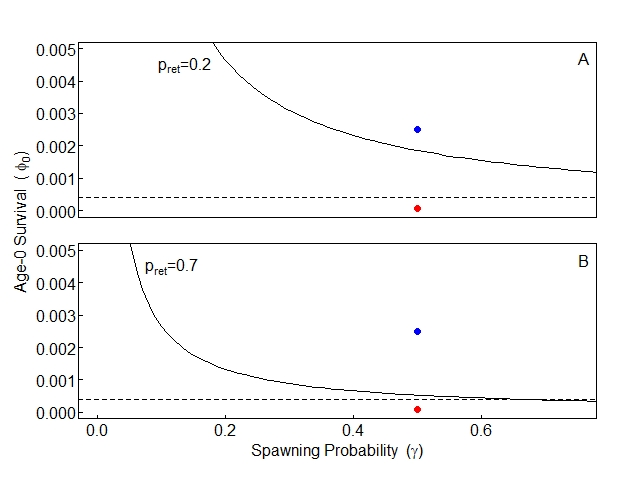
\includegraphics[width=6in]{NEPA_Fig_8-boundary-example}
\caption{Population growth-decline boundaries ($\lambda=1$) when retention probability is A) 20\% and B) 70\%.  All dots indicate a population whose reproductively-ready females spawn in the Missouri River 50\% of the time, i.e., $\gamma=0.5$.  Red dots indicate a population where 75 out of every 1,000,000 eggs are expected to survive to age-1 given retention in the free-flowing Missouri River ($\phi_0=0.000075$), and blue dots indicate a population where 25 out of every 10,000 eggs are expected to survive to age-1 given retention ($\phi_0=0.0025$).  Red dots are in a region of decline (below and left of the curve), while blue dots are in a region of growth (above and to the right of the curve).  The dashed line indicates Pine et al.'s (2001) upper estimate of age-0 survival for gulf sturgeon, 0.0004.  Population growth at this survival level can occur but only at high spawning and retention probabilities.}
\label{boundaryEx}
\end{figure}

\begin{figure}[h]
\centering
\hspace*{-0.5in}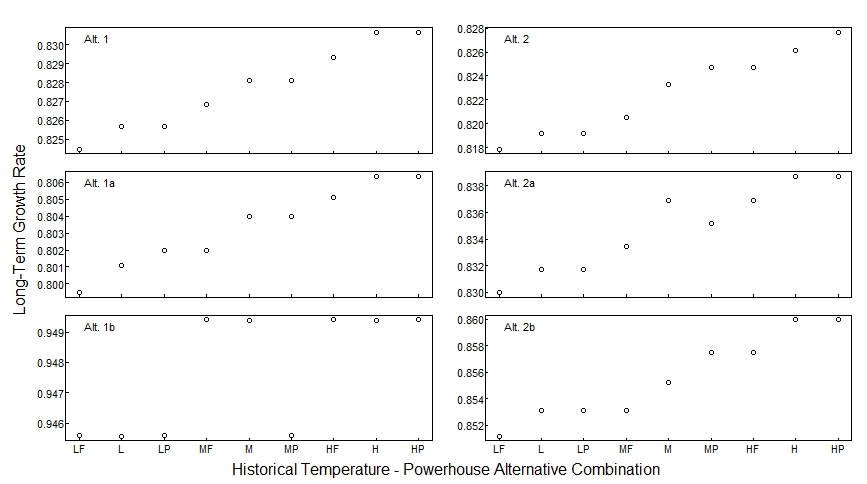
\includegraphics[width=7.5in]{NEPA_Fig_9-Year85-SA}
\caption{Long-term growth rate ($\lambda$) values for six Fort Peck flow scenarios under particular historical temperature and powerhouse operation combinations: LF--low water temperature, full powerhouse operations; L--low water temperature, standard powerhouse operations; LP--low water temperature, peak time powerhouse operations, and similar for M--median water temperature and H--high water temperature.  \textit{Check:  Median water temperatures were taken over the historical period of record (years), while low and high water temperatures were estimated as the lower and upper 95\% confidence intervals.} Full powerhouse operations assume 14kcfs are run through the powerhouse 24 hours a day; standard powerhouse operations assume 14kcfs are run through the powerhouse for 12 hours a day with 7kcfs running through the powerhouse the remaining 12 hours; peak time powerhouse operations assume 7kcfs are run through the powerhouse except during peak times (\textit{times here}) when 14kcfs are run through.}
\label{SA85}
\end{figure}

\begin{figure}[h]
\centering
\hspace*{-0.5in}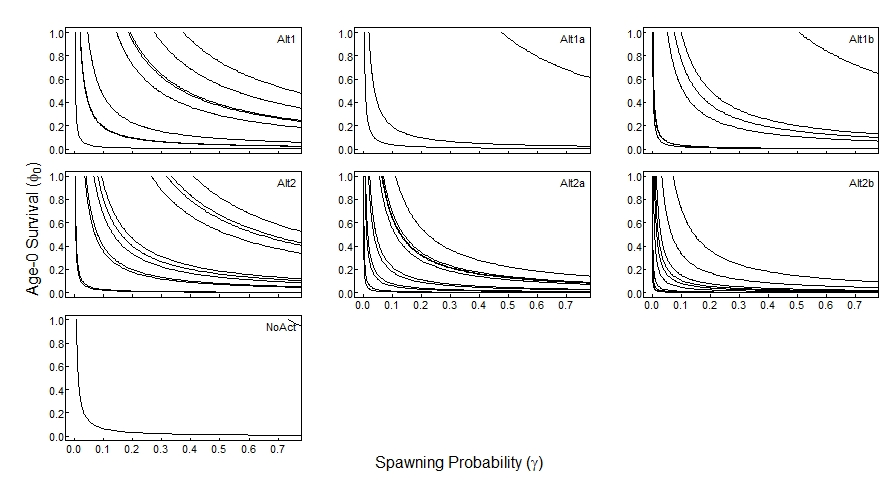
\includegraphics[width=7.5in]{NEPA_Fig_10-boundaries-year-within-alternative}
\caption{Growth decline boundaries by alternative management scenario.  Each contour line has a fixed retention probability that was computed form HEC-RAS outputs and represents a particular year in which the given alternative scenario met the flow criteria.   For a given year/retention probability, a population is expected to grow if spawning and age-0 survival probabilities fall in the space above and to the right of the curve, or, decline if spawning and age-0 survival probabilities fall in the space below and to the left of the curve. Spawning probability ($\gamma$) is the probability that a reproductively-ready female spawns in the Missouri River (vs. spawning in the Yellowstone or not spawning and reabsorbing her eggs).  Age-0 survival ($\phi_0$) is the probability of surviving from egg to age-1 given retention in the free-flowing Missouri River.}
\label{YwiA}
\end{figure}

\begin{figure}[h]
\centering
\hspace*{-0.5in}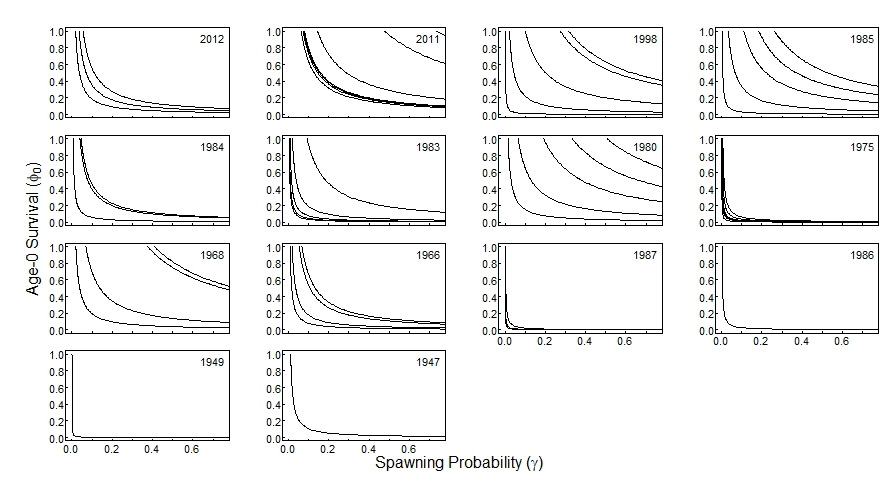
\includegraphics[width=7.5in]{NEPA_Fig_11-boundaries-alternatives-within-year}
\caption{Growth decline boundaries by year.  Each contour line has a fixed retention probability that was computed form HEC-RAS outputs and represents a particular management scenario that met the flow criteria during the given year.   For a given management scenario/retention probability, a population is expected to grow if spawning and age-0 survival probabilities fall in the space above and to the right of the curve, or, decline if spawning and age-0 survival probabilities fall in the space below and to the left of the curve. Spawning probability ($\gamma$) is the probability that a reproductively-ready female spawns in the Missouri River (vs. spawning in the Yellowstone or not spawning and reabsorbing her eggs).  Age-0 survival ($\phi_0$) is the probability of surviving from egg to age-1 given retention in the free-flowing Missouri River. }
\label{AwiY}
\end{figure}



\end{document}